\documentclass[letterpaper,twocolumn,10pt]{article}
\usepackage{usenix,epsfig,endnotes}

%%%%%%%%%%%%%%%%%%%%%%%%%%%%% DELETE AFTER %%%%%%%%%%%%%%%%%%%%%%%%%%%%%%%%%%%%
\usepackage{lipsum}
\usepackage{xargs}                      % Use more than one optional parameter in a new commands
\usepackage[pdftex,dvipsnames]{xcolor}
\usepackage[colorinlistoftodos,prependcaption,textsize=tiny]{todonotes}
\newcommandx{\unsure}[2][1=]{\todo[linecolor=red,backgroundcolor=red!25,bordercolor=red,#1]{#2}}
\newcommandx{\change}[2][1=]{\todo[linecolor=blue,backgroundcolor=blue!25,bordercolor=blue,#1]{#2}}
\newcommandx{\info}[2][1=]{\todo[linecolor=OliveGreen,backgroundcolor=OliveGreen!25,bordercolor=OliveGreen,#1]{#2}}
\newcommandx{\improvement}[2][1=]{\todo[linecolor=Plum,backgroundcolor=Plum!25,bordercolor=Plum,#1]{#2}}
\newcommandx{\thiswillnotshow}[2][1=]{\todo[disable,#1]{#2}}
\setlength{\marginparwidth}{2cm}
%%%%%%%%%%%%%%%%%%%%%%%%%%%%%%%%%%%%%%%%%%%%%%%%%%%%%%%%%%%%%%%%%%%%%%%%%%%%%%%%%
\usepackage[none]{hyphenat}
\let\origref\ref
\def\ref#1{\textbf{\origref{#1}}}







%%%%%%%%%%%%%%%%%%%%%%%%%%%%%%%%%%%%%%%%%%%%%%%%BEGIN%%%%%%%%%%%%%%%%%%%%%%%%%%%%%%%%%%%%%%%
\begin{document}

%don't want date printed
\date{}
\title{\Large \bf Towards Fog-aware Kubernetes}
\author{
{\rm Ali J. Fahs}\\
Univ Rennes, CNRS, IRISA\\
ali.fahs@irisa.fr
\and
{\rm Guillaume Pierre}\\
Univ Rennes, Inria, CNRS, IRISA\\
guillaume.pierre@irisa.fr
}
\maketitle
\thispagestyle{empty}


\subsection*{Abstract}
Your Abstract Text Goes Here.  Just a few facts.Whet our appetites.
Keep it short. According to the APA style manual, an abstract should be between 150 to 250 words Keep it short. According to the APA style manual, an abstract should be between 150 to 250 words Keep it short. According to the APA style manual, an abstract should be between 150 to 250 words  According to the APA style manual, an abstract should be between 150 to 250 words Keep it short. According to the APA style manual, an abstract should be between 150 to 250 words 
%%%%%%%%%%%%%%%%%%%%%%%%%%%%%%%%%%%%%%%%%%%%%%%%%%%%%%%%%%% INTRODUCTION %%%%%%%%%%%%%%%%%%%%%%%%%%%%%%%%%%%%%%%%%%%%%%%%%%%
\section{Introduction}
%The introduction of Fog computing. DONE
In a world where centralized data centres have been proven to be cost-effective, the big players of cloud services are relaying on more than a few data centres to serve millions of users all-over the globe. 

Such a model have seen the light due to the lack of interest in locating the services in a specific geolocation. 

 The user's applications can run in any server regardless of the location, and the communication between the user and the server is done through internet connections.\unsure{maybe i will remove this} The location of the data centres are chosen according to some factors like power cost, disregarding the impact on the end-to-end latency of the service. Furthermore, the cloud service user is not informed about the location of the server, where this location awareness is sometimes vital for specific types of application {\em (e.g., IoT applications)}.\change{language check and rephrase}

%The separation was not limited to the management alone, but also to the geographical location. 

Nowadays, some applications require lower latencies and location awareness. These requirments will be provided by an extended extended paradigm of cloud computing called Fog computing\cite{bonomi2011connected,Bonomi:2012:FCR:2342509.2342513}.

%The resource Fog provide.
The Fog computing is defined as an intermediary platform between the end devices and the cloud computing data centres. This platform provides compute, storage and networking resources,similar to clouds. Yet, the difference lies in the proximity to the user, low latency, distribution, and location awareness. 

%Fog targeted application and user proximity.
Unlike clouds which relies in a handful of resources rich data-centres, fog is based on the idea of spreading plenty points of presence in the proximity of the user. Since the end devices are close to the source, the latency can be significantly reduced, which will improve the users' experience. All of this can be done while considering the location of the access point as an important measure of the workload scheduling.

%Platforms for fog.
Since the concept of fog is relatively new, no platform was designed to assist fog architecture. However, a fog computing cluster can be deployed on top of cloud platforms like Docker swarm, Mesos, and Kubernetes.

%Kubernetes and Clouds.
For our cluster we have chosen Kubernetes for the reasons that will be mentioned in the paper.\change{link para}

%Why Kubernetes is not compatible with Fog computing (briefly).
Although Kubernetes provide automation and some source of load-balancing, still it doesn't have all the features to full-fill the definition of fog computing.    

%paper objective 
In this paper, we contribute a roadmap toward enabling a fog-aware Kubernetes.\change{definitely rephrase!}


%Explain organization of the report, what is included, and what is not.
This paper is organised as follows. In section \ref{plat} we briefly acknowledge the possible fog computing platforms. In section \ref{kube} we introduce Kubernetes as a platform, discuss the advantage and disadvantages in the context of fog. In section 
\ref{road} we demonstrate our vision through a roadmap of the steps that should be taken to achieve fog-aware Kubernetes. In the last section we conclude.\change{add something to the conclude}\unsure{long style style is ok ?} 


%%%%%%%%%%%%%%%%%%%%%%%%%%%%%%%%%%%%%%%%%%%%%%%%%%%%%%%%%%% Fog Computing %%%%%%%%%%%%%%%%%%%%%%%%%%%%%%%%%%%%%%%%%%%%%%%%%%%
\section{Fog Computing Platforms}\label{plat}
\lipsum[20]
%%%%%%%%%%%%%%%%%%%%%%%%%%%%%%%%%%%%%%%%%%%%%%%%%%%%%%%%%%% Kubernetes %%%%%%%%%%%%%%%%%%%%%%%%%%%%%%%%%%%%%%%%%%%%%%%%%%%
\section{Kubernetes and Fog Computing}\label{kube}

\subsection{Kubernetes Architecture}

\info{image will be changed}
\begin{figure}[th]
\begin{center}
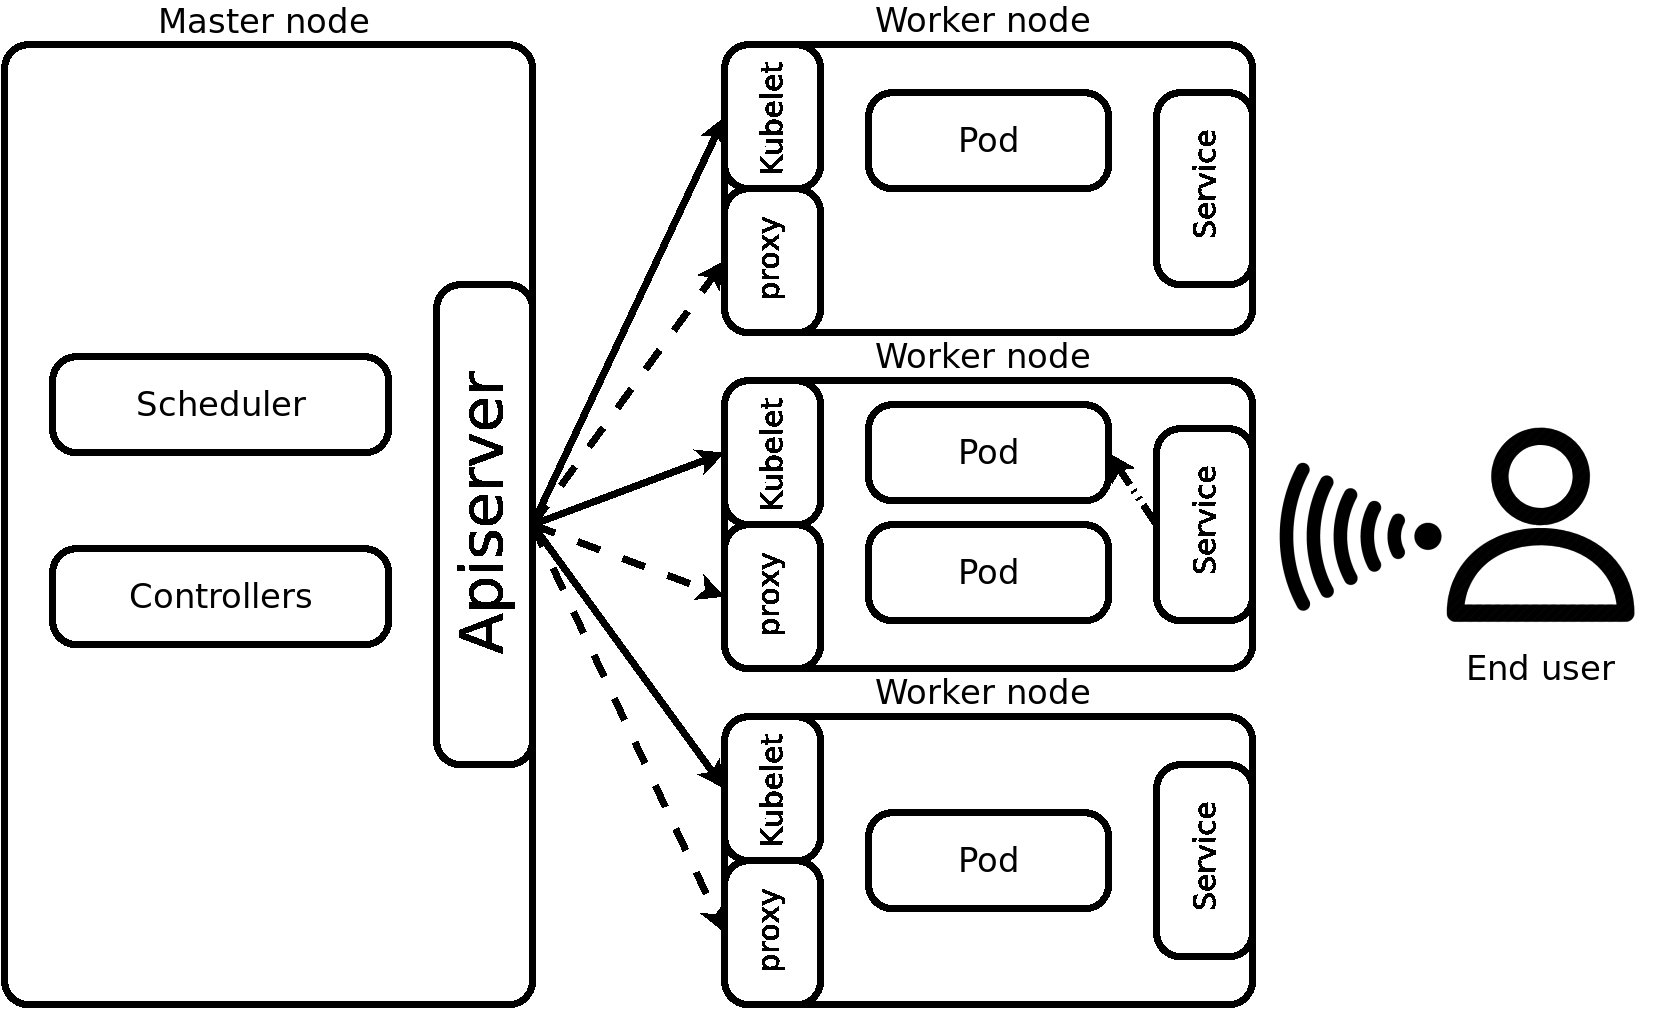
\includegraphics[width=\textwidth/2]{images/arch.png}
\end{center}
\caption{Wonderful Flowchart}
\end{figure}

%paragraph linking
Kubernetes is an open-source container-based platform created by Google, this platform manages the orchestration of the service instances. A Kubernetes cluster consist of one master node and worker nodes, where a node does not necessarily refer to a physical machine, it can also be virtual. The master node is responsible for the management and monitoring of the cluster, the master node contain the deployment scheduler and controllers. \change{rephrase!} Meanwhile, the worker nodes are the actual resources of the platform, they run the user application inside containers created by the master node. 

In the following paragraph we will refer to the master node as master and the worker node as node. 

%pods.
%deployment controllers.
Kubernetes runs containers in the form of pods, where a pod is a group of one or more containers. If a pod is consisting of more than one container, those containers can communicate internally using an isolated network\unsure{maybe it's over detailed}. The pods are created using a deployment controller located in the master node, and here we have to mention that the user is responsible of creating the deployment not the pods themselves. The automation in Kubernetes is responsible for the creation of the associated pods.

The master can schedule the pods in any of the available nodes. The pods have to communicate between each others and with users. Those communications are carried away using: 

\begin{itemize}
	\item Apiserver and Kubelet for the pod-to-pod communication.
	\item Apiserver and Kube-proxy for the communication with the user, through Kubernetes services.\improvement{shall we use k8's instead of kubernetes?}
\end{itemize}
%services
\info{add a figure of service here}

The main purpose of the service is connecting the users to exposed pods, by redirecting them to an available pod. The user will send the request to the service Ip address, then the service will choose one of the pods available in a resource pool\change{I will look for the correct name}\change{rephrase!} and looks for the Ip address of the pods in the Iptables. This selection is done in a random way or by using a load-balancer that will select the least used pod.

\info{a flow chart of the redirecting process}


\subsection{Kubernetes Advantages}

%Community.

%Scalability.

%Containerized.

%Clean separation between the app and the system.

%Distribution
\subsection{Kubernetes Disadvantages}

%Centralization.

%Location awareness.

%Bad load balancing allocations doesn’t consider the latency.

%Scheduling regardless the location.

%%%%%%%%%%%%%%%%%%%%%%%%%%%%%%%%%%%%%%%%%%%%%%%%%%%%%%%%%%% Roadmap %%%%%%%%%%%%%%%%%%%%%%%%%%%%%%%%%%%%%%%%%%%%%%%%%%%
\section{A Roadmap Towards Fog-aware Kubernetes}\label{road}

\subsection{The Decentralization}
\subsection{Location Awareness}
\subsection{Scheduling Schemes}

%%%%%%%%%%%%%%%%%%%%%%%%%%%%%%%%%%%%%%%%%%%%%%%%%%%%%%%%%%% Conclusion %%%%%%%%%%%%%%%%%%%%%%%%%%%%%%%%%%%%%%%%%%%%%%%%%%%
\section{Conclusion}

%%%%%%%%%%%%%%%%%%%%%%%%%%%%%%%%%%%%%%%%%%%%%%%%%%%%%%%%%%% Acknowledgments %%%%%%%%%%%%%%%%%%%%%%%%%%%%%%%%%%%%%%%%%%%%%%%%%%%
\section{Acknowledgments}

A polite author always includes acknowledgments.  Thank everyone,
especially those who funded the work. 

\section{Availability}


%\theendnotes


{\footnotesize \bibliographystyle{acm}
\bibliography{bibtex}
\newpage
\listoftodos[Notes]




\end{document}







